\subsection{Identifiability in the benchmark}\label{sec:val-ident}

Section~\ref{sec:identifiability} claims that the survival data pin $\eta$, $\eps$ and the mean removal $\beta\rbar$ and
leave $\kappa$ on a ridge. Three stored studies test it: the likelihood along $\kappa$ on a panel of simulated
cohorts, the calibration cost of pinning $\kappa$ (the kfix variant), and how often the released calibrator declines to
report $\kappa$ on the reference run. The first two were run on earlier versions of the benchmark library (v1 and v5) than the
reference run of Section~\ref{sec:val-benchmark} (v6); Figure~\ref{fig:ident} says which.

\paragraph{The likelihood along the ridge.} A panel of \C{kfix-panel-n} pure cohorts simulated from the SR model with
true $\kappa$ between \C{kfix-panel-ktrue-lo} and \C{kfix-panel-ktrue-hi} (\C{kfix-panel-valid} of them passing the library's validity
audit) was fitted on library v1 with $\kappa$ pinned at each of \C{ridge-n-kappa0} values from $10^{-3}$ to $300$, the other three
parameters free. On \C{ridge-valley-n} of the \C{ridge-valley-of} valid cohorts the maximised log-likelihood of every slice lay
within $1.92$ nats of the best (Figure~\ref{fig:ident}B): the data cannot choose between values of $\kappa$ that span more than
five decades. The exception has a slice that is \C{ridge-span-max} nats below the best; there the optimiser stopped at a
worse local optimum for one pinned value (a stale optimiser stop of the kind noted for the free fit), so the likelihood of that slice is a lower bound on its true value. Along the slices, raw $\beta$ moved by a median of
\C{ridge-drift-beta} decades, the removal at the threshold by \C{ridge-drift-kp1}, the mean removal $\beta\rbar$ by
\C{ridge-drift-rbar}, and $\eta$ and $\eps$ by \C{ridge-drift-eta} (Figure~\ref{fig:ident}A,C). The drift of $\beta/(1+\kappa)$ is
close to the factor of $2$ that Eq.~\eqref{eq:ridge} gives for its range (\C{ident-log2} decades).

\begin{figure}[t]
\centering
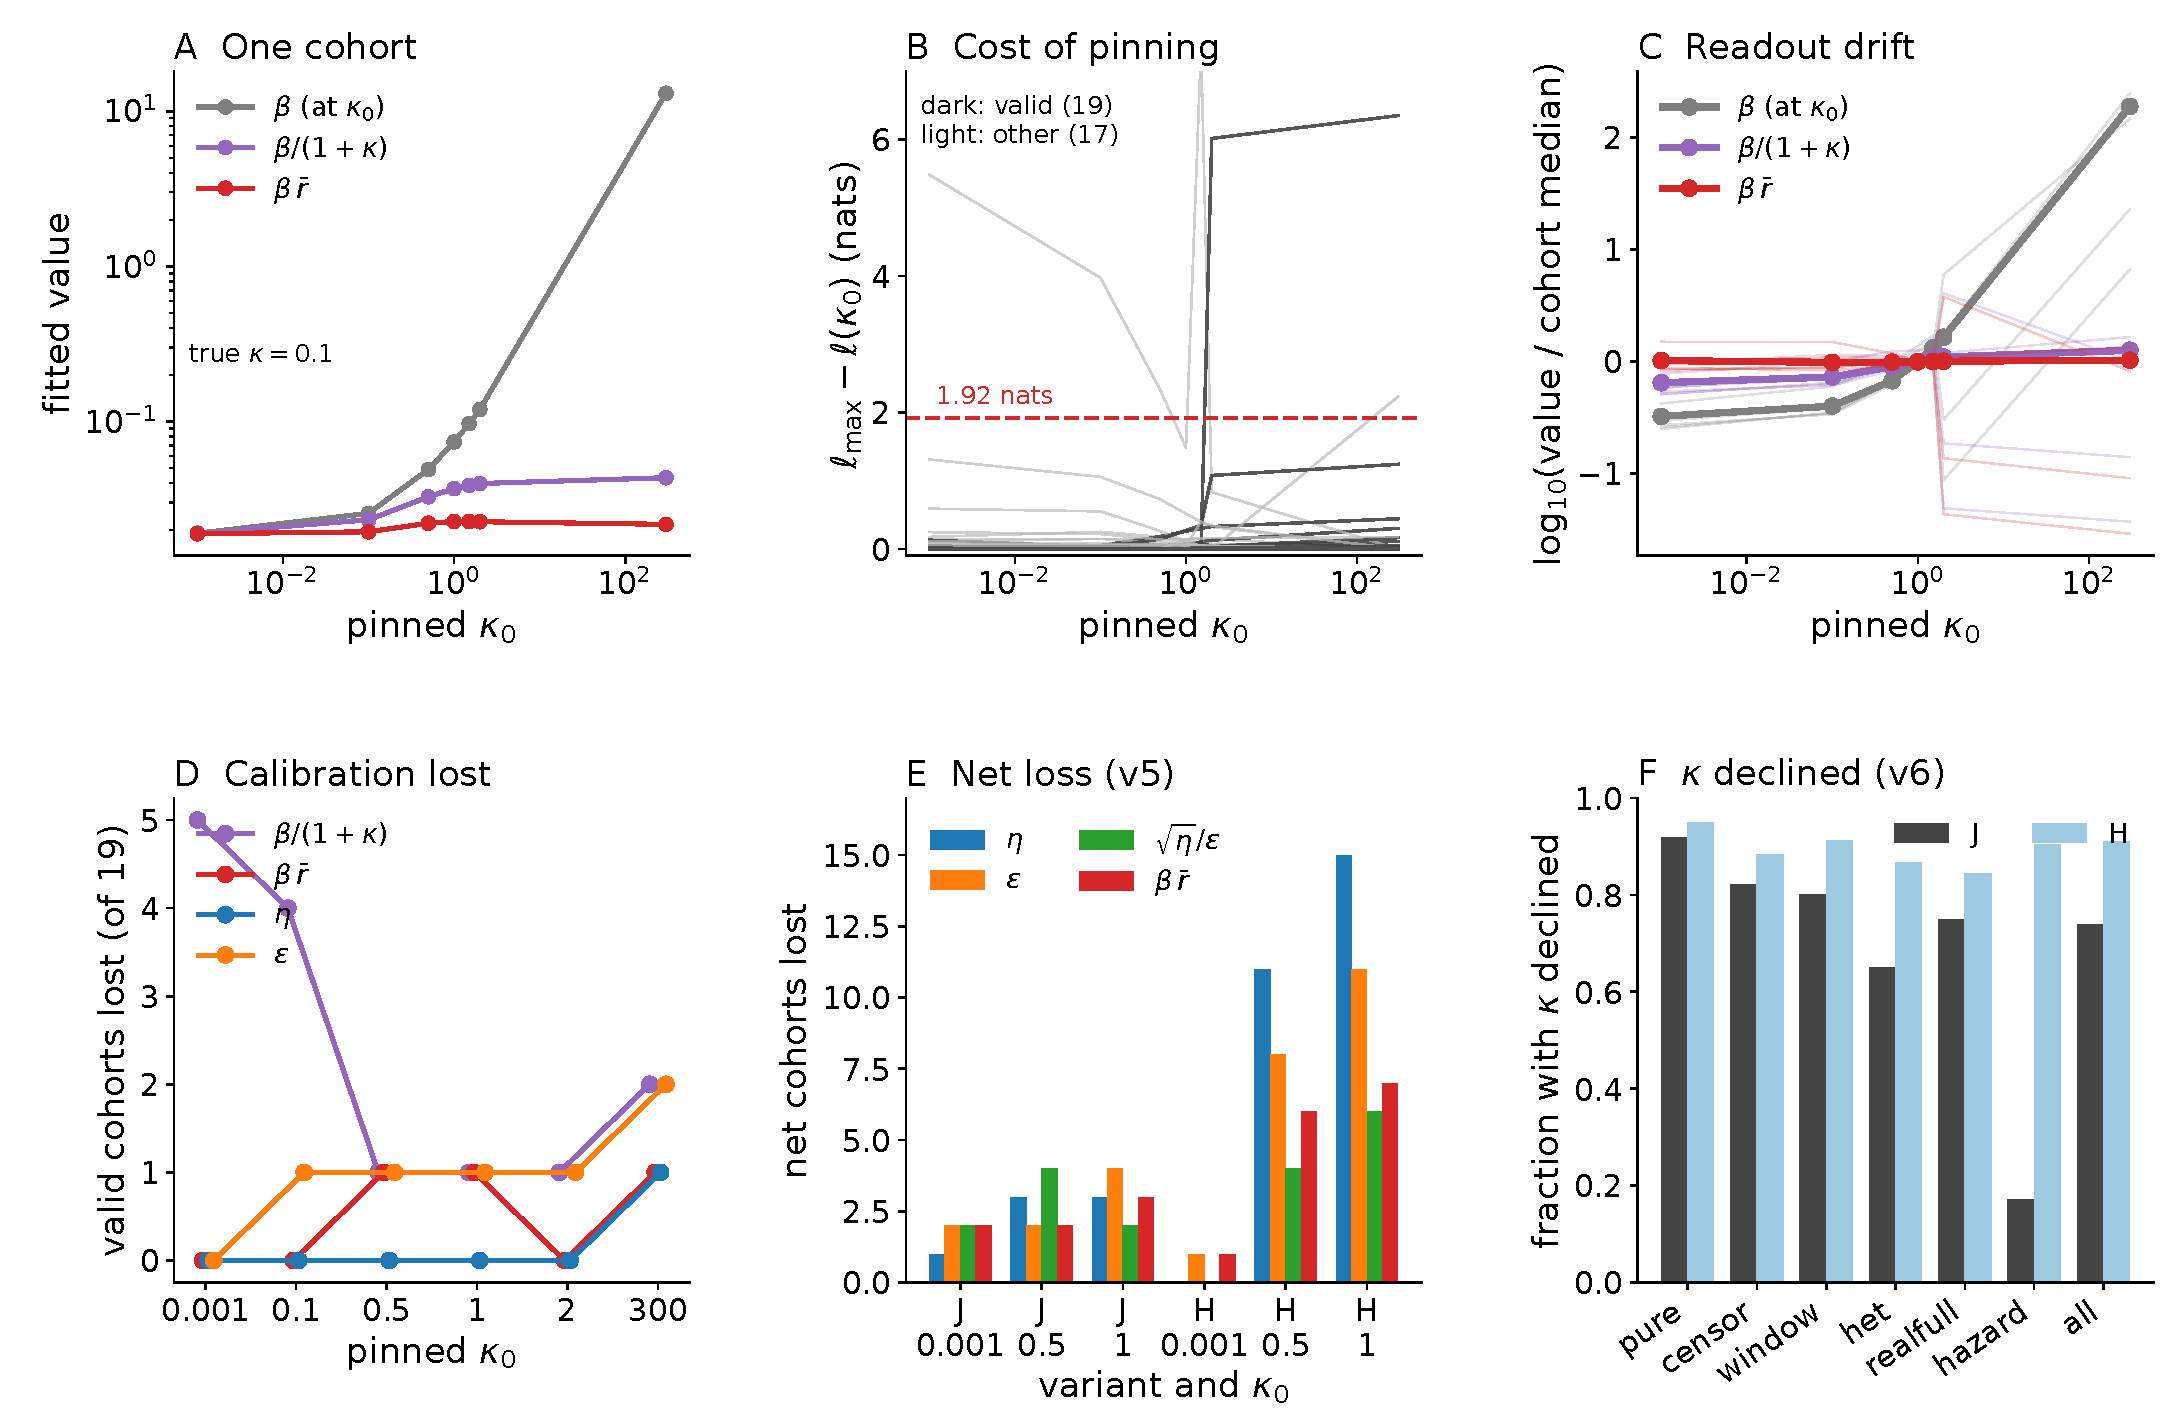
\includegraphics[width=\textwidth]{fig_ident.pdf}
\caption{Identifiability in the benchmark. \textbf{A}--\textbf{D}, panel of \C{kfix-panel-n} pure cohorts (kfix 0.1.2 on
library v1), $\kappa$ pinned at seven values $\kappa_0$. \textbf{A}, fitted $\beta$ (grey), $\beta/(1+\kappa_0)$
(purple) and $\beta\rbar(\kappa_0)$ (red) for one valid cohort with true $\kappa=0.1$; the last is nearly constant while
raw $\beta$ moves by about three decades. \textbf{B}, log-likelihood below the best slice for each cohort (dark: the
\C{kfix-panel-valid} valid cohorts); the dashed line is $1.92$ nats. Spikes are slices where the optimiser appears to have stopped at a worse local
optimum. \textbf{C}, value of each read-out relative to the median over slices, on the \C{ridge-c-n} valid cohorts whose median
mean removal is at least $10^{-3}$ (thin: cohorts; thick: median). \textbf{D}, valid cohorts lost against the free-$\kappa$
fit (of \C{kfix-panel-valid}). \textbf{E}, net cohorts lost against the free-$\kappa$ calibrator on the medium tier (library v5; $J$:
\C{kfix-J-n} paired cohorts, $H$: \C{kfix-H-n}, with \C{kfix-H-n-comb} for the two combinations), for the three released
pinned values. \textbf{F}, fraction of cohorts of the reference run (version 1.0.1, library v6, \C{gate-v6-n} cohorts) for which
$\kappa$ is declined, by arm.}\label{fig:ident}
\end{figure}

\paragraph{What pinning costs.} The kfix variant pins $\kappa=\kappa_0$ and reports $\beta$ as ``$\beta$ at $\kappa_0$'' and
the mean removal $\beta\rbar(\kappa_0)$; it declines $\kappa$ on every cohort. Against the free-$\kappa$ calibrator on
the panel, the calibration lost is small for $\eta$, $\eps$ and $\beta\rbar$ at every $\kappa_0$ and largest for
the removal at the threshold, which is lost on \C{ident-kp1-lost-k0001} of the \C{kfix-panel-valid} valid cohorts at
$\kappa_0=10^{-3}$ (Figure~\ref{fig:ident}D). On the medium tier of library v5 (paired cohort by cohort with the free-$\kappa$ run of the
released calibrator), pinning $\kappa_0=10^{-3}$ in the
released calibrator J lost a net of \C{kfix-J0001-net-eta} cohort of \C{kfix-J-n} for $\eta$, \C{kfix-J0001-net-eps} for
$\eps$ and \C{kfix-J0001-net-sqrt} for $\sqrt\eta/\eps$ and for the mean removal, gained none on $\eta$, $\eps$ or $\beta\rbar$,
and used \C{kfix-J0001-cpu} of the CPU time of the free fit (Figure~\ref{fig:ident}E). This was within the
acceptance envelope set before the run. A pinned value far from the truth costs more: at $\kappa_0=1$ the
net loss was \C{kfix-J1-net-eta} for $\eta$ and \C{kfix-J1-net-eps} for $\eps$. The variant with an external hazard
(H) is more sensitive: at $\kappa_0=10^{-3}$ it lost a net of \C{kfix-H0001-net-eta} for $\eta$ and \C{kfix-H0001-net-eps}
for $\eps$, but at $\kappa_0=0.5$ it lost \C{kfix-H05-net-eta} for $\eta$ and \C{kfix-H05-net-eps} for $\eps$ of \C{kfix-H-n}
cohorts, and at $\kappa_0=1$ \C{kfix-H1-net-eta} and \C{kfix-H1-net-eps}, which the acceptance rule classed as a loss. This
is why $10^{-3}$, which is also the saturating limit ($\rbar\approx1$), is the recommended pinned value. Reading removal at the threshold costs more than reading the mean:
in the earlier kfix study, on \C{kfix-medium-n} valid medium cohorts pinned at $\kappa_0=1$, \C{kfix-medium-kp1-lost} lost calibration for $\beta/(1+\kappa)$
against \C{kfix-medium-rbar-lost} for $\beta\rbar$, \C{kfix-medium-eps-lost} for $\eps$ and \C{kfix-medium-eta-lost} for $\eta$, with
none gained for the removal quantities.

These figures come from earlier versions of the benchmark library (v1 for the panel, v5 for the released pinned
variants); the pinned variants were not rerun on library v6, the benchmark of Section~\ref{sec:val-benchmark}
(Section~\ref{sec:limitations}).

\paragraph{How often $\kappa$ is declined.} On the reference run the released calibrator declined $\kappa$ (no claim, not even a bound) on
\C{v6-J-kappa-declined} of \C{gate-v6-n} cohorts, \C{ident-kappa-declined-pct}\,\%, and on \C{v6-J-pure-kappa-declined-pct}\,\% of the pure
arm (Figure~\ref{fig:ident}F); the exception is the arm with an external hazard, where it declined on only
\C{v6-J-hazard-kappa-declined-pct}\,\%. Variant H, which fits an external hazard, declined on
\C{v6-H-kappa-declined-pct}\,\%. Where it did report a bound, the bound was not a $95\,\%$ bound: pooled over all arms the
one-sided $\kappa$ bounds of J covered the truth in \C{ident-onesided-kappa-pct}\,\% of cases and the one-sided $\beta$
bounds in \C{ident-onesided-beta-pct}\,\%, and those of H in \C{ident-H-onesided-kappa-pct}\,\% for $\kappa$ (the reference run is
described in Section~\ref{sec:val-benchmark}; the pooled figure includes misspecified arms). The identified quantities of
Section~\ref{sec:identifiability} are the ones that carry the calibration.

The released calibrator does not store its profile along $\kappa$ in the records of the reference run, so the ridge
is drawn from the pinned-variant panel on library v1 (Figure~\ref{fig:ident}A--C) rather than from v6 cohorts.
